\documentclass[12pt]{article}
\usepackage{amsmath, amsthm, amssymb, pdfpages} 
\usepackage{fullpage}
\usepackage{hyperref}
\usepackage{graphicx}
\usepackage[capitalize]{cleveref}


\title{Test the Effectiveness of Principal Components in Adjusting for Relatedness in Genetic Association Studies}

\author{Alex, Yiqi }





\usepackage{color}
\newcommand{\myred}[1]{{\color{red} #1}}



%%% To set proper spacing
\usepackage[vcentering,dvips]{geometry} 
\geometry{papersize={8.5in,11in},total={6.5in,8.5in}} 
\renewcommand{\baselinestretch}{1.15}
\begin{document}
	\maketitle
	
	
\section{Introduction} 

Genome-wide association study (GWAS) has been widely used to investigate whether target Single Nucleotide Polymorphism (SNP) is associated with certain trait (association study). However, considering admixture population is involved in recent study, linkage disequilibrium (LD) exists due to the chromosomal segments of different sub-population's (k) ancestry [1]. The existence of linkage disequilibrium or failure to correct for population structure can reduce statistical power. Hence, principal component analysis (PCA) which is a dimensionality-reduction method is used to provide examination for admixture population to identify the causal locus [2,3]. Although in recent study PCA has been a standard method to investigate the GWAS, doubts are cast on its statistical power when comparing with other existing implementation such as linear mixed model (LMM) [4]. Since current studies mainly focus on simple simulations or observation on real data [4, 5], existing evaluation can be limited to fully investigate the statistical power of PCA. In this paper, both simulation and real data set are used to evaluate the performance of PCA under different situations.\\

According to the result of our simulation, 

\section{Method} 
\subsection{Theory connecting to kinship}

\subsection{PCA GWAS  is Equivalent to linear regression with covariate}
The original model in our project has the same structure to linear regression. We assume that in this model, there are n individuals and m genetic marker. The formula can be written as: $$Y=\mu+X \vec{\beta}+\vec{\epsilon}$$. Here, Y is a n*1 vector which represents trait value for each individual and X is a n*m genotype matrix. In addition, $\vec{\beta}$ and $\vec{\epsilon}$ are a n*1 vectors representing the coefficient of genetics marker and residuals separately. Here $\epsilon$ follows a normal distribution $N(0,\sigma)$. This model sometimes fails beacause the number of genetic market is much larger than the number of indivudual. Then, we introduce PCA to make approximations\\

In a PCA linear regression model, we can write it in the form of $$y=\mu+ \vec{X_{j}} {\beta}_{j}+U_{1:i} \nu+\vec{\epsilon}$$

Here Y still repesents the numerical value of trait of different individual and $\mu$ is the intercept. Both of them are n*1 vector. Meanwhile, $\vec{X_{j}}$ is a n*1 vector of $j_{th}$ genetic marker and in this csae, $\beta$ is a scale regression coefficient. Then, $U_{1:i}$ is a n*i matrix which is the first i Principal Components and $\nu$ is a n*1 coefficient vector for $U_{1:i}$. In the end, $\epsilon$ represnets the residual which follows a normal distribution $N(0,\sigma)$ which is the same to previous model. Then, we need to test the significance of each gemetic marker. The null hypothesis is ${\beta}_{j}$ equals to 0 and the model in this case can be written as $y=\mu+U_{1:i} \nu+\vec{\epsilon}$ for $j_{th}$ market. The alternative hypothesis is ${\beta}_{j}$ does not equal to 0. Therefore, we will conduct the F test to investigate whether the reduced model can have the same statistical power. If the p-values is small, which indicates this market is associated with trait.\\

In our simulation, each individual will be test 100000 SNPs (Single Nucleotide Polymorphism) and each for each loci (in total 100000), we will conduct linear regression separately.  The genotype of each loci will be combined with eigenvector of principal components matrix which is composed of eigenvectors we used in PCA.Regarding the eigenvector of principal component, it is calculated by decomposing the kinship matrix.  

\subsection{Admixture Simulation}
The construction of admixture population is mainly based on admixture simulation of Alex (2016). The related code of admixture simulation has been uploaded to Github with a R package called "bnpsd".  Some parameters are changed in order to better simulate under different situation. According to Alex (2016), the number of independent loci is 30000, in this paper the number of independent locus is 10000. The default value of Alex (2016) is 3, whereas in this project, it can be variable. Considering the difference among number of sub-population, the sample size of $i_{th}$ sub-population will be set as the smaller integer of the ratio of total sample divided by number of sub-population.\\
Regarding the family structure, the generation will be set to be 20 to simulate admixture population with the existence of family structure. Considering the large calculation cost during the generation process of admixture population with family structure, this data set will be treated as real data set. It will be used repeatedly to test performance of PCA under different situations with random traits.



\subsection{Trait Simulation}
The construction of trait simulation is based on a R package called "simtrait". This package constructs the complex trait simulation with user-defined causal loci and the desirable heritability of the trait. It can be used in both simulated data set and real data set if the kinship matrix is estimated correctly. \\
In our simulation,the function of trait can be written as $$y=G+ \epsilon$$ 
, where G represents the effect of genotype and $\epsilon$ represents the noise.  The noise follows a normal distribution with mean zero and variacne  equals to one minus hertability rate times desired parametric variance factor of the trait which is 1 in default. To obtain the genotype effect, marginal allele frequency will be calculated first and then, SNP will be randomly selected as causal index with random SNP coefficients. Then  coefficients of causal index will be scaled and centered to estimate the genotype effect, thereby obtaining the numerical value of traits of each causal loci.


\subsection{Result Examination Method}
In this paper, precision-recall curves and uniformity p-value test will be used to test the performance of PCA under different scenarios. Both two methods will be illustrated by boxplot.
\subsubsection{Precision-Recall Curves}
Precision-recall curve is a plot whose y-axis represents precision and x-axis represents recall. Precision is calculated as the number of true positives divided by sum of both true positives which indicates the performance of model in predicting positives. Similarly, recall measures the ratio of number of true negatives and sum of true negatives and false negatives, which measures the performance of model in predicting negatives.Hence, the precision measures the relevancy of result which indicates the proportion of selected items are relevant. The recall shows the proportion of relevant items are selected. The precision and recall curve demonstrates the trade-off among precision and recall. Hence, the formula of precision and recall can be written as:
$$Precision=\frac{True Posotive}{True Positive+Flase Positive}$$
$$Recall=\frac{True Posotive}{True Positive+Flase Negative}$$

The area under the curve (AUC) is calculated as the integration of curve of precision and recall. It measures the aggregated performance of through different thresholds. The range of AUC is from 1 to 0. When AUC equals to 1, it can be interpreted as the predictions of model is $100\%$ correct, whereas, AUC equals to 0 indicates that all predictions of this model are wrong. 
\subsubsection{Uniform P-Value Test }
Due to the existence of multiply hypothesis test in our simulation, the frequency of erroneous inferences will increase. Altough Bonferroni Correction can be used to deal with this problem, it can result in high false negative rate (FNR). The better strategy is to controlling the False Discovery Rate (FDR). FDR is calculated as the ratio of flase positives and the sum of true positives and false positives.For multiple independent and identical hypothesis tests, if the null hypothesis is true, the distribution of p-values will approximate to a uniform distribution [8]. In this case, a bette strategy is to use the q-value rather than p-value to control the FDR. Therefore, we should evaluate the performance of PCA by quantifying the distribution of p-value of null hypothesis. If distribution of p-vlaues of null hypothesis is significantly deviates from the quantiles of uniform distribution, the resulting q-values are anti-conservative.Thus, we use root mean square deviation (RMSD) to measure the fittness of quantiles p-values to the expected quantiles of uniform distribution. The RMSD is calculated as the root of mean square of the difference among sorted p-values of null hypothesis and expected quantiles of sorted p-values of null hypothesis after removing causal indexes.The numerical values of RMSD is inversely  performance of PCA. The formula of RMSD is:
$$RMSD=\sqrt{\sum{(p_{uniform}-p_{null}})^2}$$
where $p_{null}$ is a list of p-values of null hypothesis after removing causal index and $p_{uniform}$ is a list of expected quantiles of $p_{null}$ in uniform distribution. \\

In many other papers, genomic control is another popular approach to detect the existence of population stratification and written as $\lambda_{GC}$ . The definition of $\lambda_{GC}$ is median chi-square asscociation statistic which has one degree of freedom through SNPs divided by theoretical median based on the null hypothesis. Hence, if hte $\lambda_{GC}$ close to 1, it indicates that there is no or little population stratification. However, if $\lambda_{GC}$ is larger than 1 significantly, it means there exists population stratification, or other confounder factors. Genomic control $\lambda_{GC}$ only use median to measure the existence of stratification, whereas, RMSD make full use of data which should be more powerful. Hence, in this paper, RMSD is used to measure the performance of PCA in terms of p-value (type 1 error).


\subsection{Comparison among PCA and Existing Implementations }
Some current research argue that Linear Mixed Model (LMM) can outperform PCA in correcting for population strcuture. In Linear Mixed Model, population strcuture is treated as ramddom effect. In this project, LMM will be tested under the same admixture simulation and trait simulation to PCA and thus, comparison between LMM and PAC with different PCs used under different situations can be made. Additionally, PCA with no PC used is equivalent to Linear Regression (LM). We will also consider the performance comparision among PCA and LM. 

\subsection{true or biased kinship matrices has the same performance}



\section{Result}

We use simulation data where genotypes and trait will be simulated following procedure mentioned above. We first set the sample size to be 1000 and then, we reduce the sample size to 100 to investigate whether PCA still have similar performance under new scenario. We will conduct 10 times simulation so that the extra variance can be reduced. For each simulation, performance of PCA will be collected in terms of RMSD and AUC for PCs from 2 to 90. Also, real data set will also be introduced to test the performance of PCA and trait will be simulated in the same way to simulation data. Then, We will test the performance of PCA when family structure exists with sample size equals to 1000 and 100 separately. Finally, we test the performance of PCA with the existence of complex family structure and here we set the generation to be 20.

\subsection{PCA performance under N=1000}
\begin{figure}[bp!]
  \centering
  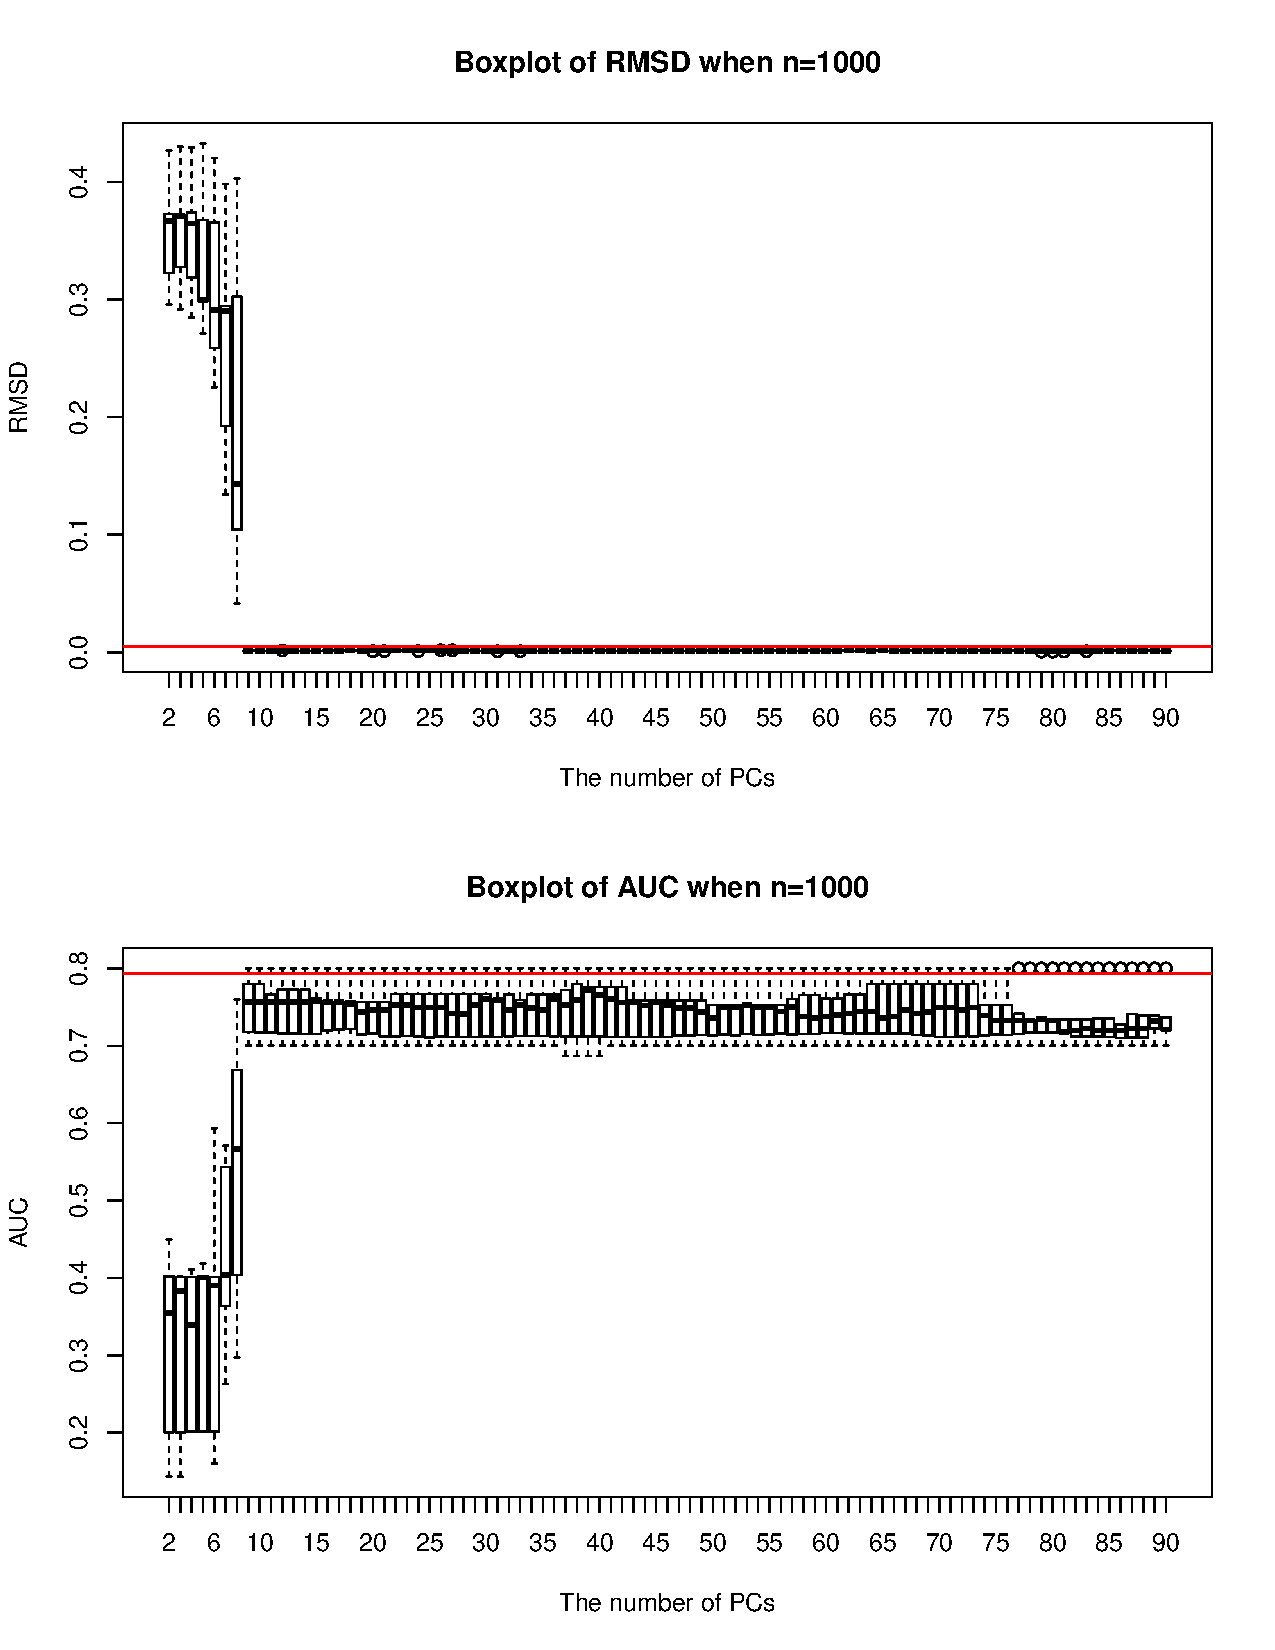
\includegraphics[width=4in]{C:/Users/yiqiy/Desktop/gas-rgls/PCA_gwas/PCA_n_1000_m_100_k_10.pdf}
  \caption{
    {\bf boxplot of rmsd and auc}
    The first panel is the boxplot of RMSD when sample size is 1000. Here the y axis represents value of rmsd and x axis is the number of PCs used in PCA.
    The second panel is the boxplot of AUC and here y axis is value of AUC. RMSD is used to measure the deviation of distribution of p values of null hypothesis from uniform distribution. In the case of multiple null hypothesis holds, the distribution of p-values of null hypothesis should approximate to unifrom distribution. Therefore, we use root mean square deviation (RMSD) to measure the deviation between the distribution of p-values and uniform distribution. The small value of RMSD implies type one error is well controlled. Regaring AUC, it's calculated by integration of predicion and recall curve. The value of AUC can be interpreted as the proportion of predictions made by this model is correct. The result of Linear Regression is put at the position of PC equals to zero and the result of LMM is put at the position of PC equals to 91.}
  \label{fig:example}
\end{figure}

According to the first panel in Figure 1 which is the boxplot of RSMD when the number of subpopulation is 10 and sample size is 1000, it can be seen that RMSD values remain relatively high when p is smaller than 9, which satisfies the actual rank of genotype matrix or kinship matrix which is (k-1). It demonstrates that the distribution of p-values of null hypothesis deviates from the expected quantiles of uniform distribution and therefore, PCA fails to control FDR.Though the performance of PCA is relatively bad, there still exists an decreasing tendency. It indicates that when the number of PCs used in PCA is smaller than true rank of genotype matrix, PCA will benefit forom using more PCs in terms of controlling FDR. However, once the number of PCs used in PCA reaches the actual rank of genotype matrix or kinship matrix, the RSDM will junmp to a small value and in this case the value of RMSD is close to 0. It remains stable as the number of PCA increases. Apart from this, it can be seen that before the number of PCs reaches the rank of genotype matrix, the distance among minimum and maximun of RMSD is larger. It tends to be smaller after number of PCs used in PCA is larger than the rank of genotype matrix, which shows less fluctuations in terms of type 1 error controlling. Compared with the performance of other existing method, it can be seen that both PCA and LMM controll type one error well once the number of PCs used in PCA is larger than the true rank of genotype.\\

The seond pandel of Figure 1 illustrates the pattern of AUC for the same scenario to the first panel. In this case, we can see a increasing tendency for AUC when the number of PCs is samller than the true rank of genotype or kinship matrix. Such a tendency indicates that the increase of number of PCs can increase predictive power of PCA when it is smaller than the rank of genotype matrix. Once the number of PCs used in PCA exceeds the rank of PCA, the value of AUC will be increased to around 0.8, which indicates that $80\%$ predictions of PCA are correct. After that, PCA does not benefit from adding more PCs as it can not increase the value of AUC obviously. Similarly, the range of AUC tends to be smaller than it when the number of PCs used in PCA is greater than rank of genotype matrix. In terms of LMM, the average AUC value is slightly higher than AUC of PCA even the number of PCs is larger than true rank of genotype matrix. \\


\subsection{PCA performance under N=1000}
\begin{figure}[bp!]
  \centering
  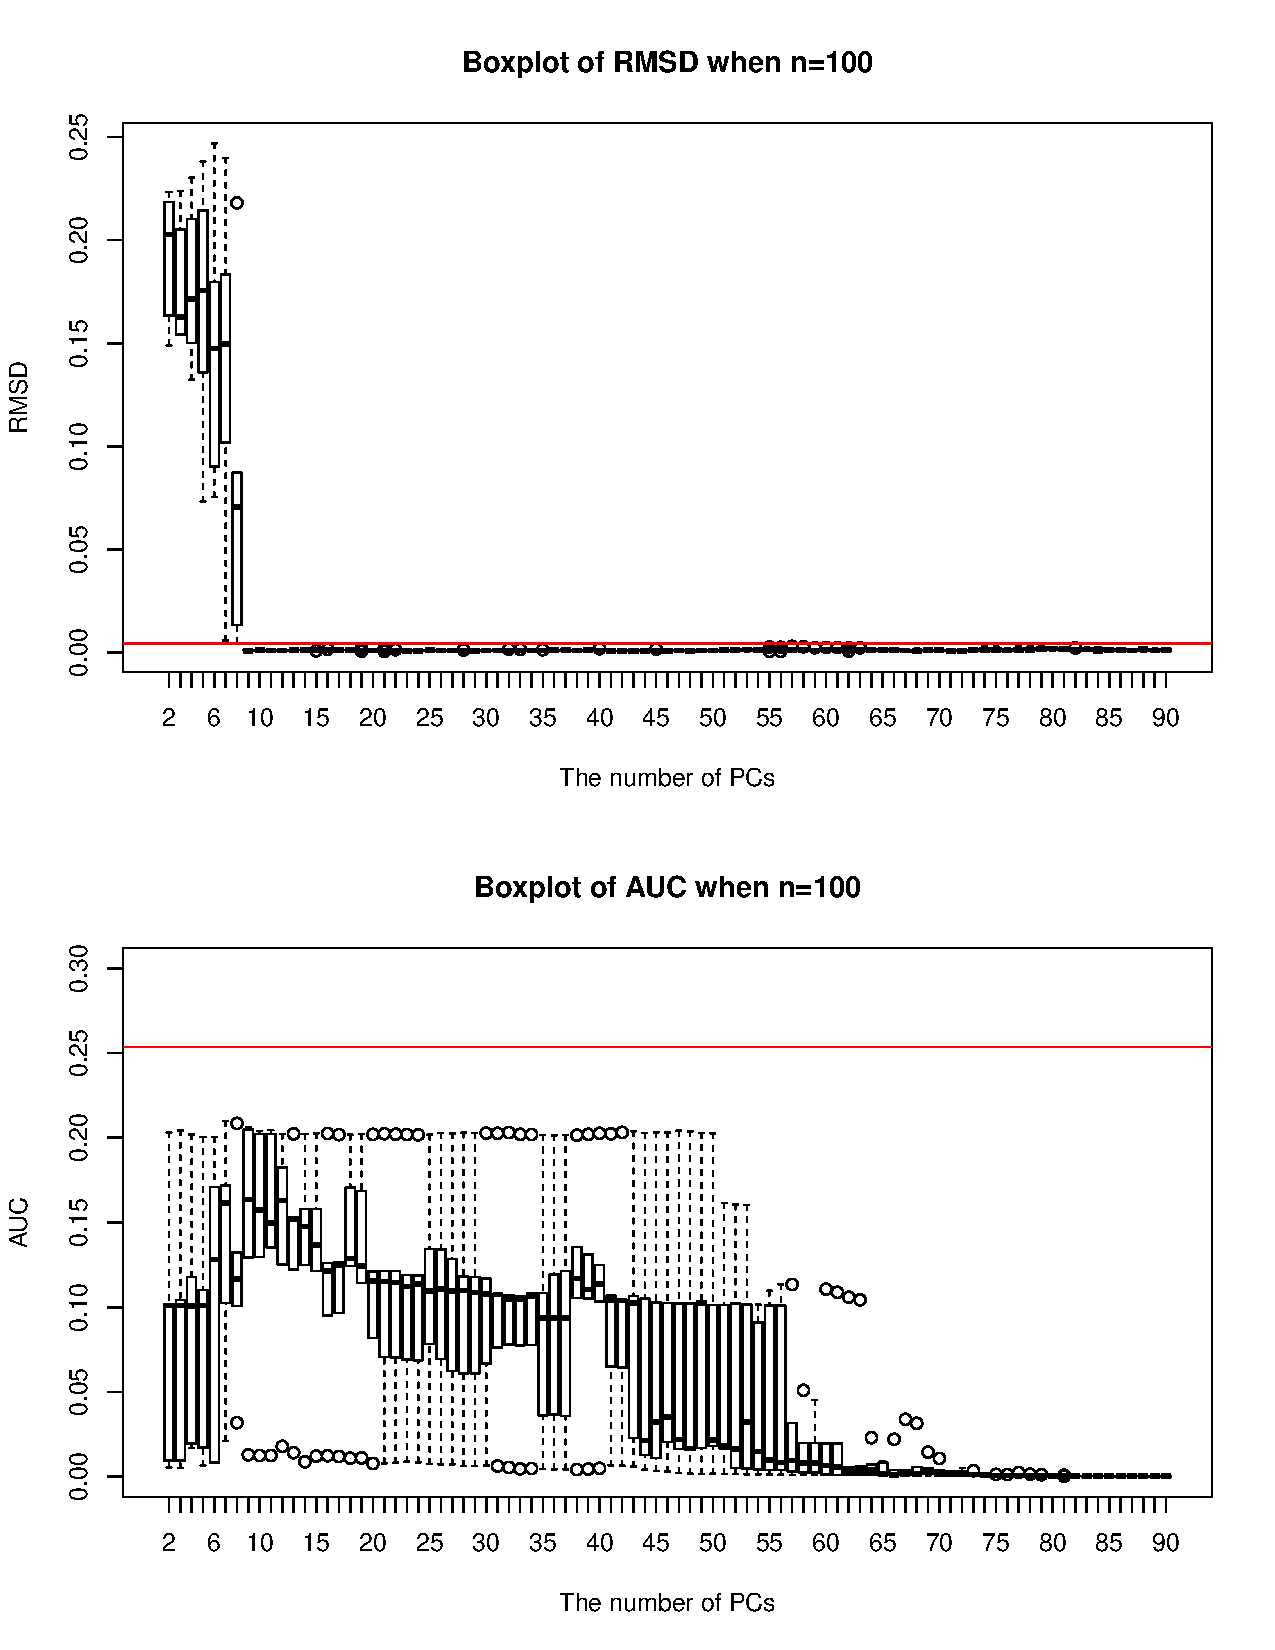
\includegraphics[width=4in]{C:/Users/yiqiy/Desktop/gas-rgls/PCA_gwas/PCA_n_100_m_10_k_10.pdf}
  \caption{
    {\bf boxplot of rmsd and auc}
    The first panel is the boxplot of RMSD when sample size is 1000. Here the y axis represents value of rmsd and x axis is the number of PCs used in PCA.
    The second panel is the boxplot of AUC and here y axis is value of AUC. RMSD is used to measure the deviation of distribution of p values of null hypothesis from uniform distribution. In the case of multiple null hypothesis holds, the distribution of p-values of null hypothesis should approximate to unifrom distribution. Therefore, we use root mean square deviation (RMSD) to measure the deviation between the distribution of p-values and uniform distribution. The small value of RMSD implies type one error is well controlled. Regaring AUC, it's calculated by integration of predicion and recall curve. The value of AUC can be interpreted as the proportion of predictions made by this model is correct. The result of Linear Regression is put at the position of PC equals to zero and the result of LMM is put at the position of PC equals to 91.}
  \label{fig:example}
\end{figure}
\subsection{PCA performance under N=100}

Then we want to investigate the performance of PCA when samlpe size is samll. Here we set the sample size to be 100. From the first panel of Figure 2, it can be seen that the pattern is similar to the boxplot of RMSD in the case of sample size equals to 1000. It illustrates an decreasing when the number of PCs is smaller than true rank of genotype matrix. It indicates that PCA can better control type 1 error in this situation. If the number of PCs is greater than true rank of genotype matrix, the RSMD will decrease immediately and approximate to zero, which shows type 1 error is excellently controlled. Hence, PCA is insensitive to the smaple size in terms of RMSD or type 1 error controlling. Moreover, the performance of LMM in this case is similar to Figure 2 which is close to previous figure. The RMSD value of LMM approximates to 0 which indicates that there is no significant difference among PCA and LMM in this csae.\\

Concerned with the boxplot of AUC, the pattern is obviously different from the boxplot of AUC when smaple size is 1000. Although we still can find an increasing pattern of AUC before the number of PCs reaches the k. However, it can be seen that there is an decreasing pattern of AUC value once the number of PCs exceeds the true rank of PCA. It demonstrates that, even though fluctuations exist, performance of PCA in terms of power can be wrose with the increase of PCs used in PCA. Furthermore, maximum value of AUC when sample size is 1000 approximate 0.8, however the maximum value of AUC when sample size is 100 is around 0.2. It illustrates that only $20\%$ predictions made by this model is correct and hence, it fails in terms of power when sample size is small. Considering LMM, the average` AUC value is 0.25, whereas, the maximum AUC of PCA is 0.2 and it decreases immediately due to the excessive use of PCs. In this case, LMM performs better than PCA in terms of power. \\




\begin{figure}[bp!]
  \centering
  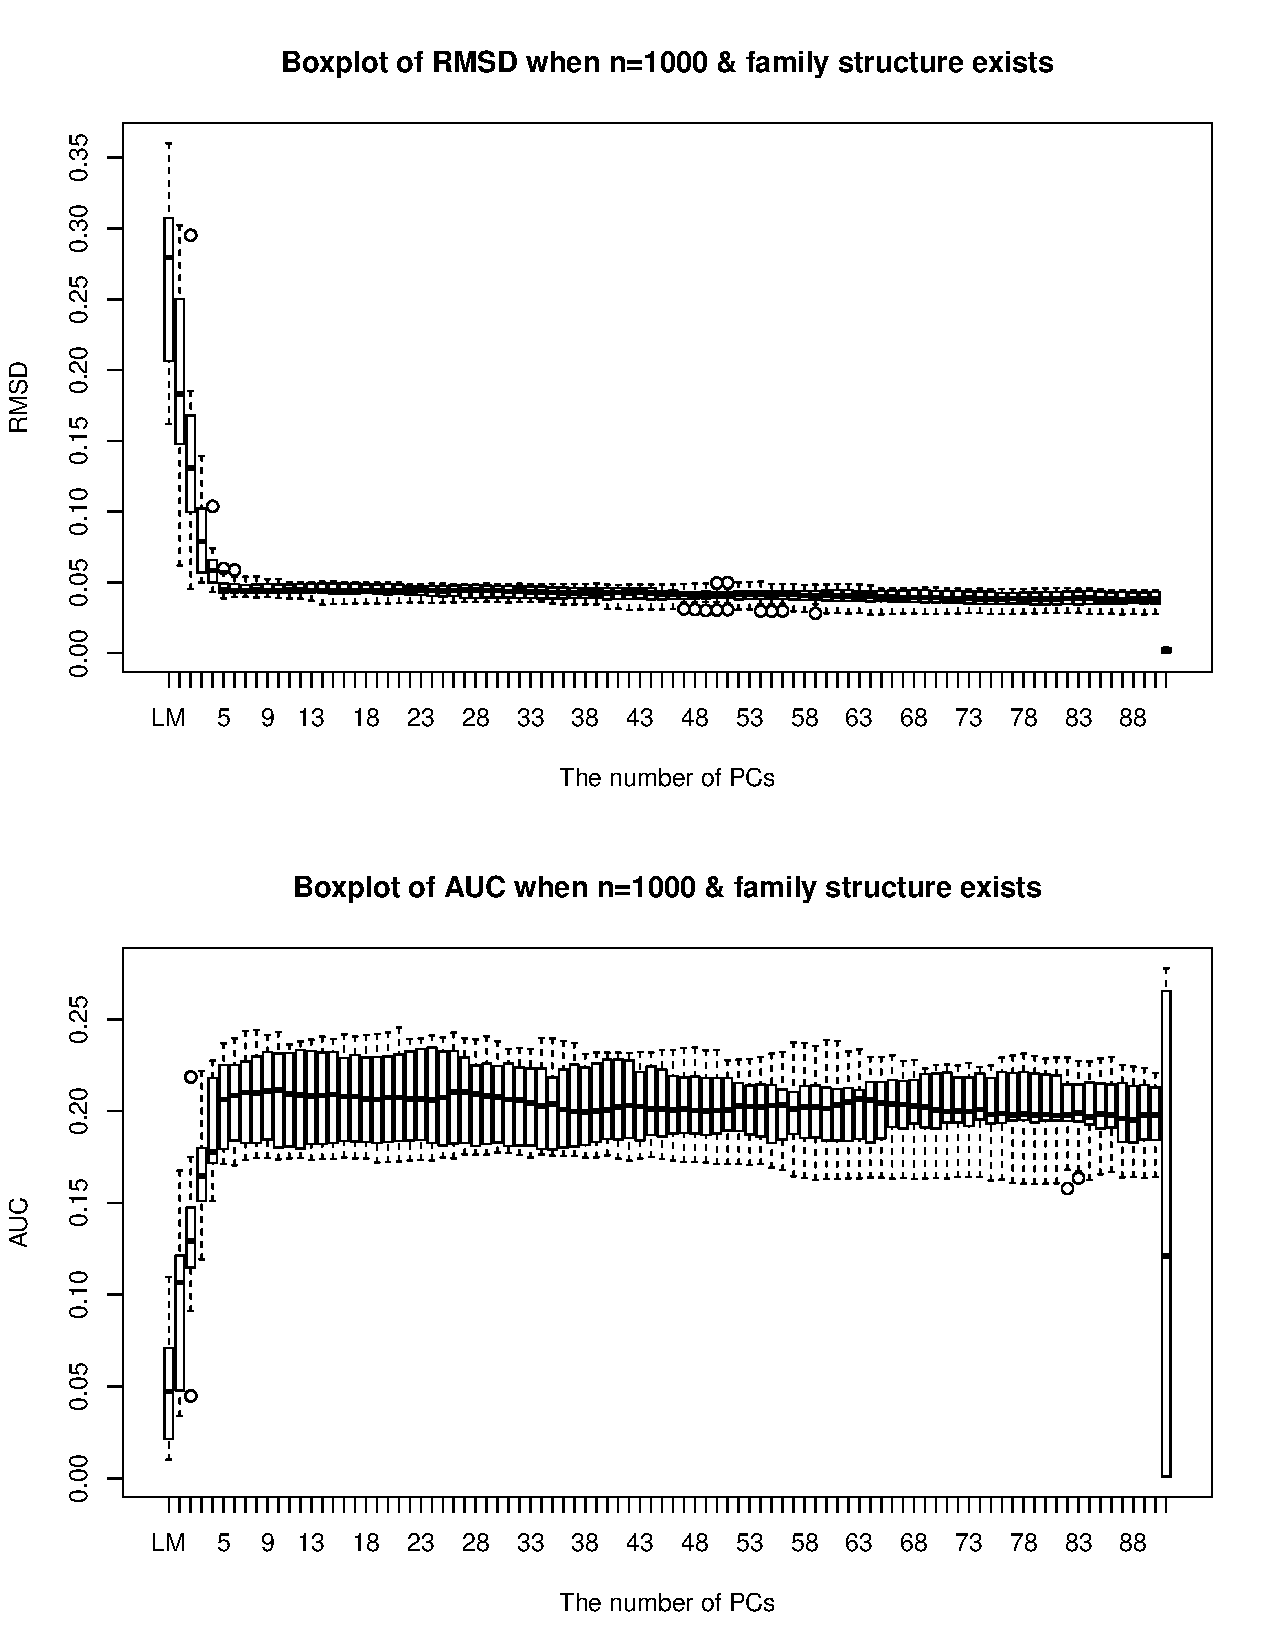
\includegraphics[width=4in]{C:/Users/yiqiy/Desktop/gas-rgls/PCA_gwas/PCA_n_1000_m_100_family_structure.pdf}
  \caption{
    {\bf boxplot of rmsd and auc}
    The first panel is the boxplot of RMSD when sample size is 100.}
  \label{fig:example}
\end{figure}

\subsubsection{PCA performance when familty structure exists}

The introduction of family structure will make the original admixture populatio more complicated. In this csae, we assume that there are 20 generations in total with other factors fixed. Based on the result of the first panel in figure 3 indicates that there is a decreasing pattern of RMSD for the first three PCs. It addition, the value of RMSD in this situation is large, which indicates that the distribution of p-value of null hypothesis does not approximate to uniform distribution. It illustrates that PCA fails to control type one error when the number of PCs is not enough. When the number of PCs is larger than 4, values of RMSD beome stable around 0.05 which demonstrates that there exists evidence of the distribution of p-value of null hypothesis does not deviate from uniform distribution but the evidence is weaker than previous simulation where RSDM approximates to 0. Considering the range of RMSD, it decreases first and then begins to increase. It shows that excessive use of PCs will lead to extra variance.For AUC, it illustrates an increasing tendency for the first three PCs. When the number of PCs is larger than 3, AUC fluctuates around 0.2. This shows the power of PCA is small and hence, PCA fails in this csae in terms of power even though enough PCs are used. 

\section{Conclusion}


Consequently, we can conclude that PCA perform poorly when the number of PCs is smaller than the ranks of genotype matrix or kinship matrix. When the number of PCs is smaller than rank of kinship matrix and genotype matrix, RMSD values will be quite high which indicates the distribution of p-values of null hypothesis significantly deviates from uniform distribution. It means PCA fails to control type 1 error. Regarding the value of AUC, it will be quite low and thus, power of PCA in this case is small. When sample size large enough and number of PCs used in PCA is no smaller than rank of genotype matrix, PCA works pretty well in both type 1 error and power. In this scenario, value of RSMD approximates to 0 and value of AUC is around 0.8. Moreover, the performance of PCA will not be improved with more PCs used. PCA is still roboust to type one error controlling in the case of small sample size, whereas, it will be punished in terms of power with excessive PCs used in PCA. Furthermore, when enough PCs are used in PCA, we will expect similar performance of PCA and LMM in terms of type one error, regardless of the sample size is large or not. However, regarding AUC, LMM outperforms PCA slightly when the sample size is large. In the case of small sample size, LMM has strong advantage over PAC in AUC, even though the AUC value of LMM is also small. 

\section{Discussion}
\subsection{PCA GWAS fails without enough PCs}
Right now, both LMM and PCA have become standard approaches to correct for admixture population. In current PCA GWAS research, the number of PCs used in PCA is assmued to be 10. Based on the simulation of Hoffman (2013), 10 PCs are randomly selected from the first 30 PCs and the performance of PCA is close to LMM when 
\subsection{PCA GWAS still works even too many PCs are used}
PCA GWAS still works even though PCs of eigenvectors are excessively used. From the box b



\subsection{PCA GWAS fails with the existence are close relatives }



\section{Reference List}
$
1
Pasaniuc, B., Zaitlen, N., Lettre, G., Chen, G. K., Tandon, A., Kao, W. L., ... \& Larkin, E. (2011). Enhanced statistical tests for GWAS in admixed populations: assessment using African Americans from CARe and a Breast Cancer Consortium. PLoS genetics, 7(4), e1001371.
$\\

$
2
Bryc, K., Auton, A., Nelson, M. R., Oksenberg, J. R., Hauser, S. L., Williams, S., ... \& Bustamante, C. D. (2010). Genome-wide patterns of population structure and admixture in West Africans and African Americans. Proceedings of the National Academy of Sciences, 107(2), 786-791.
$\\

$
3
Price, A. L., Weale, M. E., Patterson, N., Myers, S. R., Need, A. C., Shianna, K. V., ... \& Goldstein, D. B. (2008). Long-range LD can confound genome scans in admixed populations. The American Journal of Human Genetics, 83(1), 132-135.
$\\

$
4
Wang, K., Hu, X., \& Peng, Y. (2013). An analytical comparison of the principal component method and the mixed effects model for association studies in the presence of cryptic relatedness and population stratification. Human heredity, 76(1), 1-9.
$\\



$
5
Ochoa, A., \& Storey, J. D. (2016). FST and kinship for arbitrary population structures I: Generalized definitions. BioRxiv, 083915.
$

$
6
Martin, A. R., Gignoux, C. R., Walters, R. K., Wojcik, G. L., Neale, B. M., Gravel, S., ... \& Kenny, E. E. (2017). Human demographic history impacts genetic risk prediction across diverse populations. The American Journal of Human Genetics, 100(4), 635-649.
$\\



$
8
Simonsohn U, Nelson L D, Simmons J P. P-curve: a key to the file-drawer[J]. Journal of experimental psychology: General, 2014, 143(2): 534.
$
\end{document}
